\newif\ifLoneInTOC
\LoneInTOCfalse

\AddToHook{shipout/background}{%
	\ifLoneInTOC
		\begin{tikzpicture}[remember picture, overlay]
			\node[anchor=north west, inner sep=0pt, outer sep=0pt] at (current page.north west) {
				\resizebox{\paperwidth}{\paperheight}{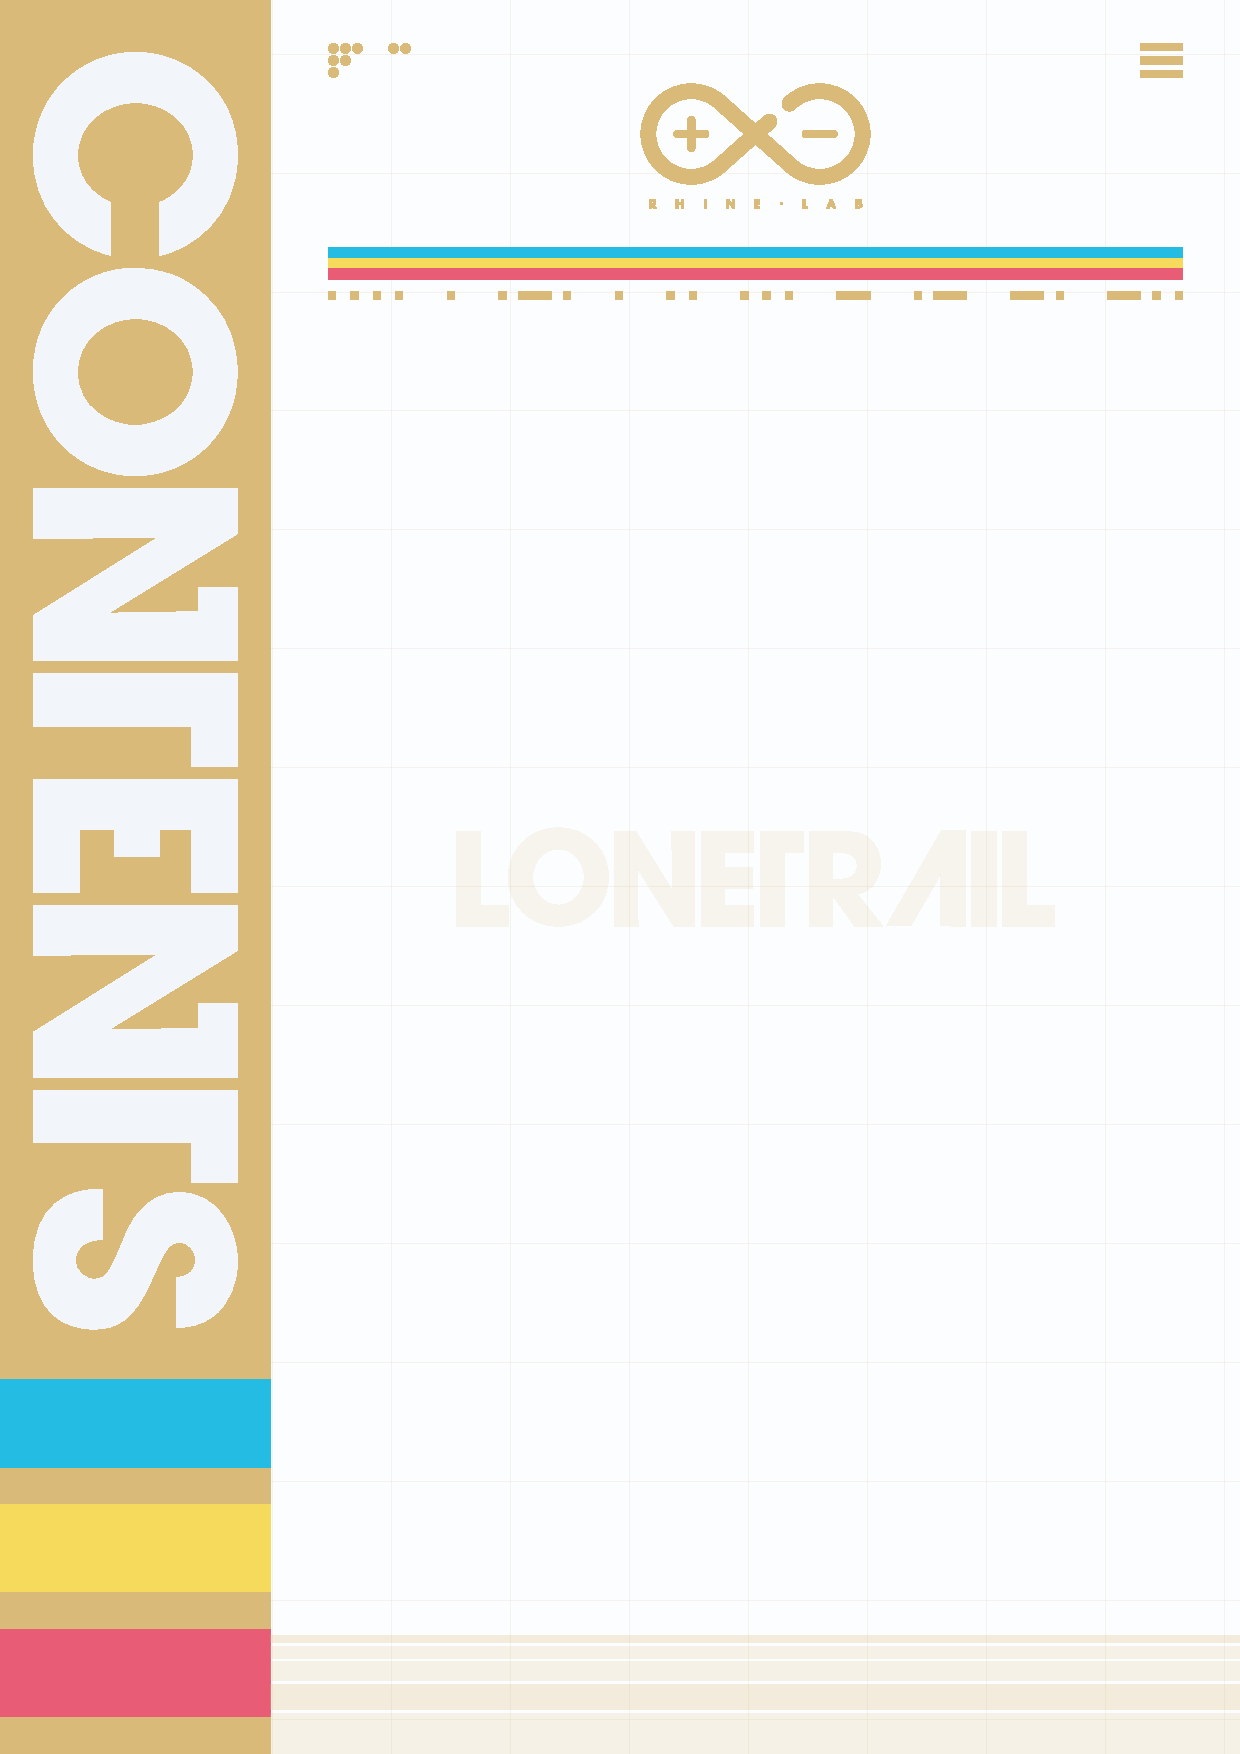
\includegraphics{assets/pdf/contents_bg.pdf}}
			};
		\end{tikzpicture}%
	\fi
}

\renewcommand{\sectionmark}[1]{\markboth{#1}{}}
\renewcommand{\subsectionmark}[1]{\markright{#1}}
\renewcommand{\contentsname}{}
\setlength{\cftbeforetoctitleskip}{0pt}
\setlength{\cftaftertoctitleskip}{0pt}
\setcounter{secnumdepth}{0}
\renewcommand{\cftdot}{}

% ---------------- 默认目录间距参数（如未在 main.tex 中定义则采用以下默认值） ----------------
\providecommand{\TOCSecSepSpace}{4.0pt}    % 1. 大标题与下方彩色短横线间距
\providecommand{\TOCSubInnerSpace}{13.0pt} % 2. 小标题内部折行间距
\providecommand{\TOCSubItemSpace}{8.5pt}   % 3. 小标题与小标题之间的间距

\makeatletter
\newlength{\TOCPageNumW}
\setlength{\TOCPageNumW}{24pt}

\renewcommand{\l@section}[2]{%
	\vspace{16pt}%
	\par\noindent
	\begin{minipage}[t]{\dimexpr\linewidth-\TOCPageNumW\relax}%
		\raggedright
		\setlength{\lineskiplimit}{-10pt}%
		\setlength{\lineskip}{0pt}%
		{\cftsecfont\ignorespaces#1\par}%
	\end{minipage}%
	\hfill
	\makebox[\TOCPageNumW][r]{{\cftsecpagefont\ignorespaces#2}}%
	\par\nointerlineskip
	\vspace{\TOCSecSepSpace}%
	\noindent
	\raggedright
	\resizebox{200.5pt}{4pt}{
\includegraphics{assets/pdf/separator_1.pdf}}%
	\par
	\vspace{6.0pt}%
}

\renewcommand{\l@subsection}[2]{%
	\par\noindent
	\begin{minipage}[t]{\dimexpr\linewidth-\TOCPageNumW\relax}%
		\raggedright
		{\cftsubsecfont\ignorespaces#1\par}%
	\end{minipage}%
	\hfill
	\makebox[\TOCPageNumW][r]{{\cftsubsecpagefont\ignorespaces#2}}%
	\par\nointerlineskip
	\vspace{\TOCSubItemSpace}%
}
\makeatother

% 原版思源黑体 CJK 定义（大标题 C 档 13.5pt，小标题由 \TOCSubInnerSpace 控制）
\setCJKfamilyfont{SiYuanTOC}[Path = ./assets/fonts/, Extension = .otf]{SiYuan}
\renewcommand{\cftsecfont}{\CJKfamily{SiYuanTOC}\SiYuan\CJKsetecglue{}\fontsize{16pt}{13.5pt}\selectfont\bfseries}
\renewcommand{\cftsecpagefont}{\CJKfamily{SiYuanTOC}\SiYuan\CJKsetecglue{}\fontsize{16pt}{13.5pt}\selectfont\bfseries}
\renewcommand{\cftsubsecfont}{\CJKfamily{SiYuanTOC}\SiYuan\CJKsetecglue{}\fontsize{12pt}{\TOCSubInnerSpace}\linespread{1.0}\selectfont\bfseries}
\renewcommand{\cftsubsecpagefont}{\CJKfamily{SiYuanTOC}\SiYuan\CJKsetecglue{}\fontsize{12pt}{\TOCSubInnerSpace}\selectfont\bfseries}

\newcommand{\makecustomtoc}{%
	\pagenumbering{gobble}%
	\pagestyle{empty}%
	\begin{adjustwidth}{100pt}{0pt}
		\begin{multicols*}{2}
			\tableofcontents
		\end{multicols*}
	\end{adjustwidth}
}

\hypersetup{linktoc=all}
